\documentclass{beamer}

\usepackage{default}
\usepackage{amssymb}
\usepackage[utf8]{inputenc}


\DeclareGraphicsExtensions{{.pdf},{.png},{.jpg}}
\graphicspath{ {./img/} }

\hypersetup{colorlinks,urlcolor=blue}
\AtBeginSection[]
{
	\begin{frame}
		\begin{NoHyper}
		\tableofcontents[currentsection]
		\end{NoHyper}
	\end{frame}
}
\begin{document}
\addtobeamertemplate{footline}{\insertframenumber/\inserttotalframenumber}

	
\title{You are the way you (structurally) talk:  Structural-temporal neighbourhoods of posts to characterize users in online forums}
\author{Alberto Lumbreras \\Jouve B., Velcin J., Guégan, M.}
\date{April 8, 2016}
\maketitle

\begin{frame}\frametitle{Overview} 
\begin{NoHyper}
\tableofcontents
\end{NoHyper}
\end{frame}

\section{Introduction}
\subsection{The data}

\begin{frame}{The data}{Reddit. A forum of forums}
	\begin{figure}
		\centering
		
\includegraphics[width=0.1\textwidth]{reddit-logo}	
	\end{figure}
	Download monthly dumps from:
	\href{http://couch.whatbox.ca:36975/reddit/comments/monthly/}{http://couch.whatbox.ca:36975/reddit/comments/monthly/}
	
	\vfill
	Extract forum of interest:\\
	\href{www.reddit.com/r/podemos}{www.reddit.com/r/{\color{red}science}}\\
	\href{www.reddit.com/r/podemos}{www.reddit.com/r/{\color{red}france}}\\
	\href{www.reddit.com/r/podemos}{www.reddit.com/r/{\color{red}sociology}}\\
	\href{www.reddit.com/r/podemos}{www.reddit.com/r/{\color{red}complexsystems}}\\
	\href{www.reddit.com/r/podemos}{www.reddit.com/r/{\color{red}podemos}} $\leftarrow$ in this presentation\\
	...
\end{frame}

\subsection{The graph representations of the data}

\begin{frame}{Graph representations}{Graph of user interactions (a social network)}
	\begin{figure}
		\centering
		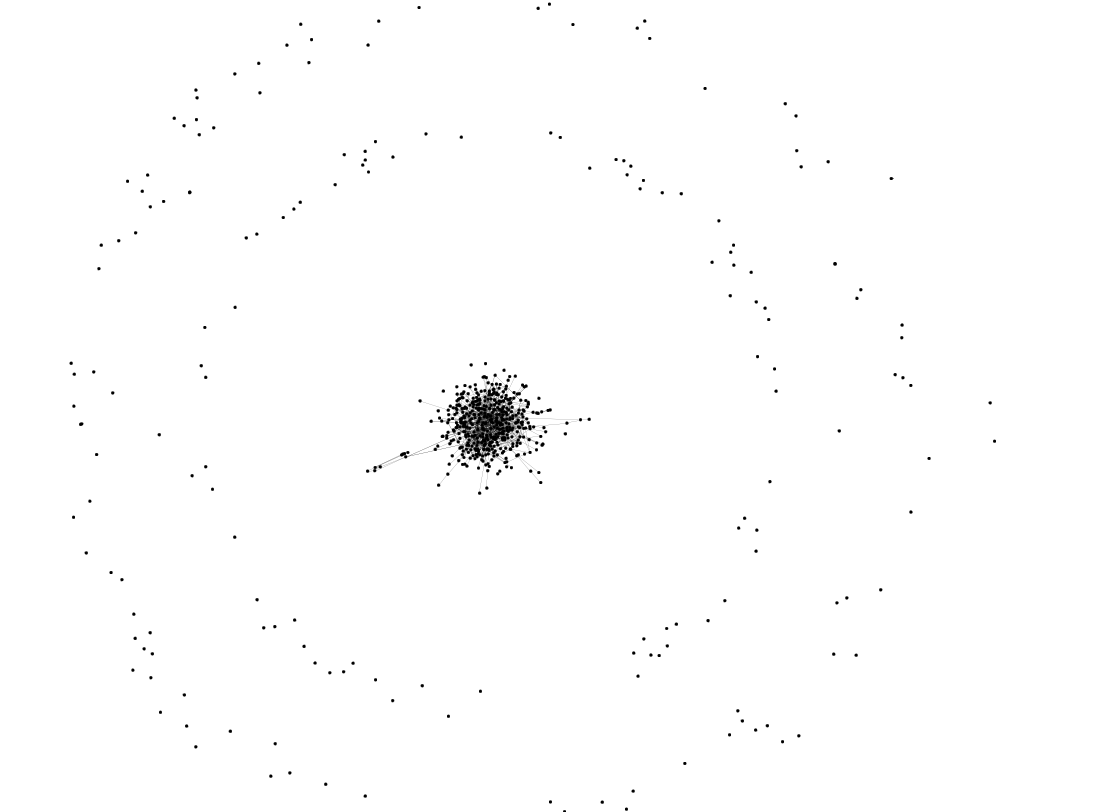
\includegraphics[width=1\textwidth]{sna}	
	\end{figure}
\end{frame}

\begin{frame}{Graph representations}{Trees of posts}
\begin{figure}
	\centering
	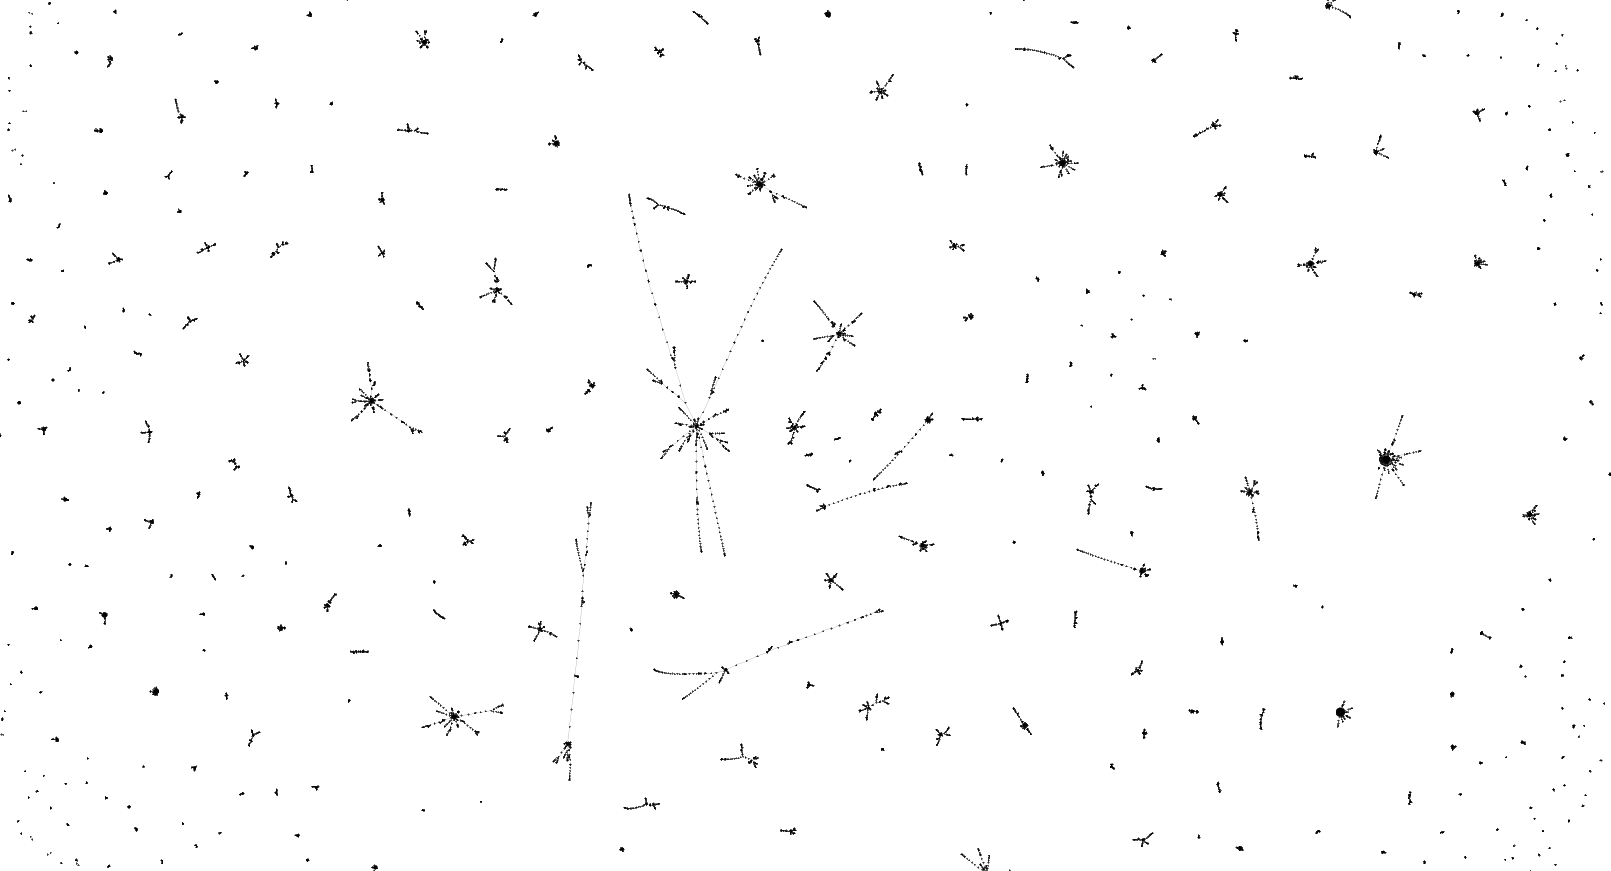
\includegraphics[width=1\textwidth]{forest}	
\end{figure}
\end{frame}

\begin{frame}{Graph representations}{Which one is better?}

\begin{itemize}
\item Depends on the task!
\item One might choose multiple representations (multi-level analysis)
\end{itemize}
\vfill
My choice: 
\begin{itemize}
\item Mostly tree representation
\item Because it explicitly represents discussions (and their evolution).
\end{itemize}
\begin{figure}
	\centering
	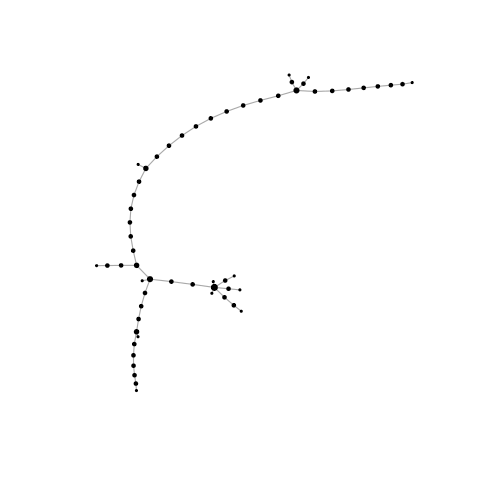
\includegraphics[width=0.3\textwidth]{tree1}	
	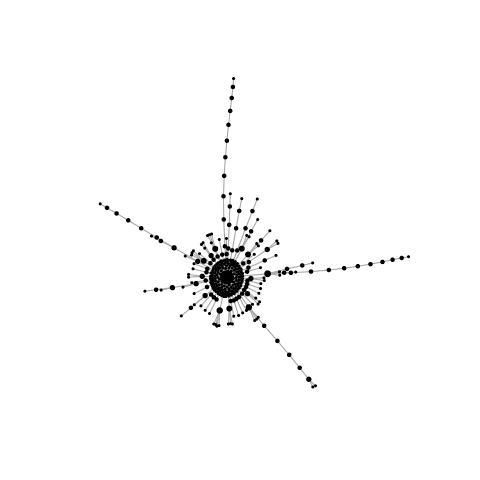
\includegraphics[width=0.3\textwidth]{tree2}	
	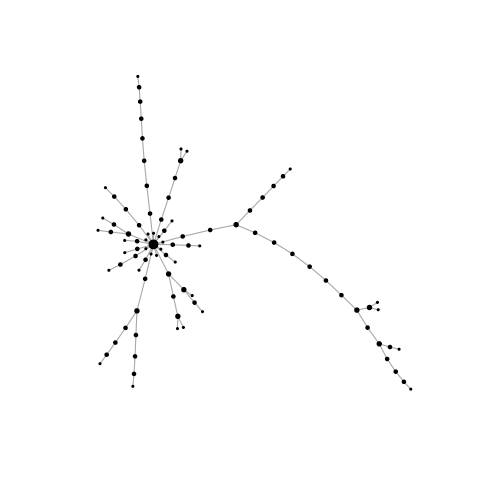
\includegraphics[width=0.3\textwidth]{tree4}	
\end{figure}
And sometimes:
\begin{itemize}
\item SNA representation of single conversations.
\end{itemize}
\end{frame}

\section{Structures of conversations}
\subsection{Basic idea}
\begin{frame}{Intuition}
\textit{Hypothesis}: different individuals have tendency towards different types of conversations and these types are reflected in the structure of their interactions.
\vfill
These conversational structures might be observed at two levels (at least):
\begin{itemize}
\item Social graph.
\item Posts graph (tree)
\end{itemize}
\end{frame}


\subsection{Triadic structures}
\begin{frame}{Triadic structures}{Triads are not enough}
	\begin{figure}
		\centering
		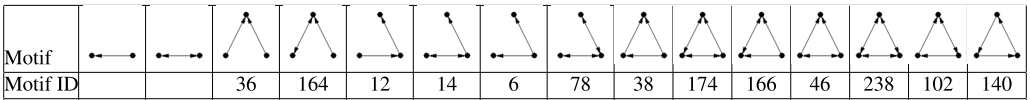
\includegraphics[width=1\textwidth]{triads}
	\end{figure}
	
Triads in \textbf{trees of posts}:
	\begin{itemize}
		\item Only 3 possible triads (dyad, chain and star)
	\end{itemize}

Triads in  \textbf{social graph}:
	\begin{itemize}
		\item Order (therefore dynamic) is missing.
	\end{itemize}
\vfill
We need something richer that captures the dynamics of conversations.
\end{frame}

\subsection{Neighbourhood structures}
\begin{frame}{Order-based neighbourhoods}{Definition}
\begin{itemize}
	\item 1. Extract neighbourhood of post $i$ with radius $r$.
	\item 2. Keep only the $n$ posts that are closest (in time) to post $i$. 
\end{itemize}
	\begin{figure}
		\centering
		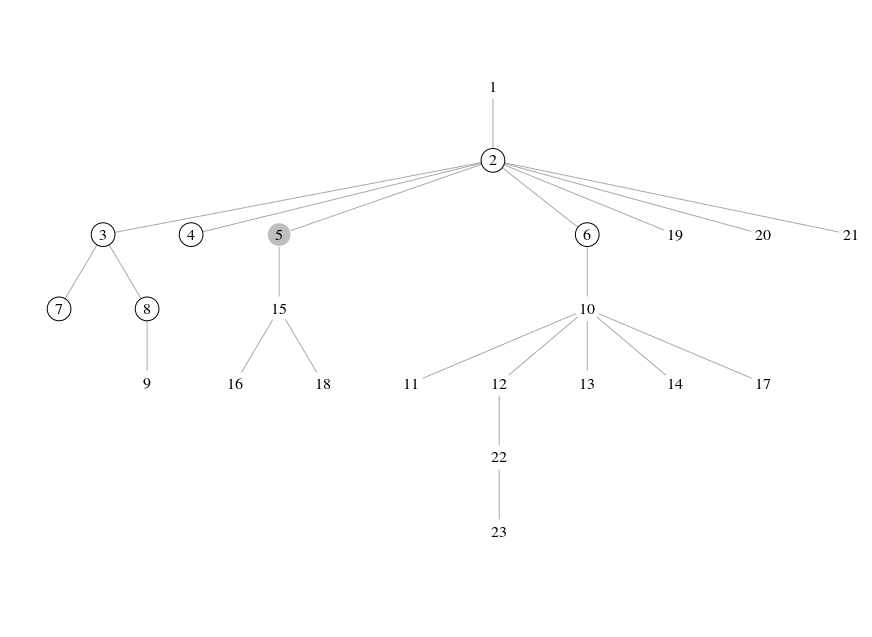
\includegraphics[width=01\textwidth]{order_neighbourhood}
	\end{figure}
Easy to compute, but how to choose the parameters $r,n$ ?  	
\end{frame}

\begin{frame}{Order-based neighbourhoods}{Census}
We found 129 different motifs:
	\begin{figure}
		\centering
		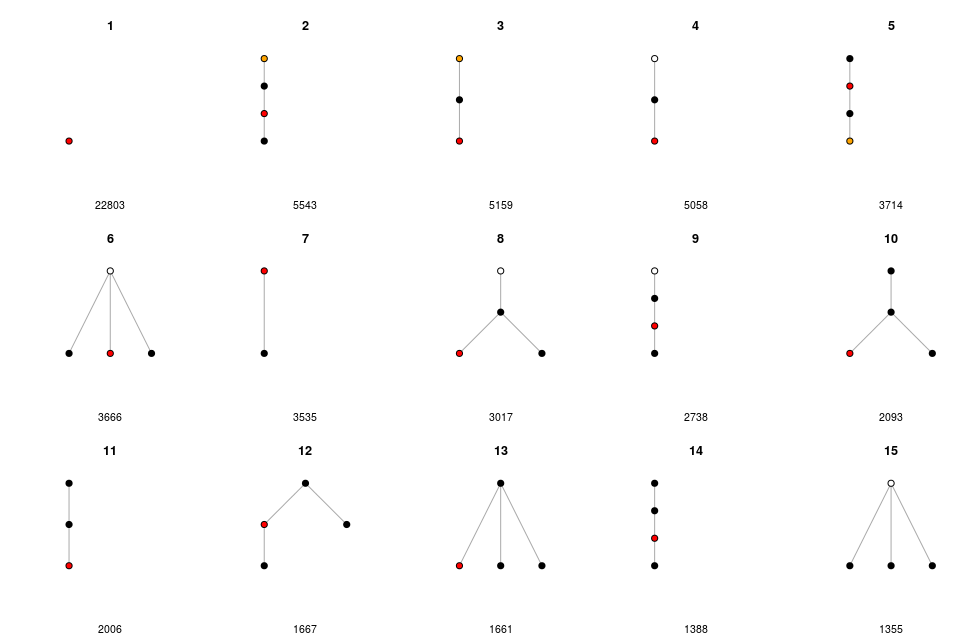
\includegraphics[width=1\textwidth]{neighbourhoods_2_4_1}
	\end{figure}
\end{frame}

\begin{frame}{Time-based neighbourhoods}{Definition}
\begin{itemize}
	\item 1. Extract neighbourhood of post $i$ with radius $r$.
	\item 2. Detect changes of speed (vertical/horizontal changepoints)
	\item 3. From $i$, get the posts around until a changepoint is found.
\end{itemize}
%\vspace{cm}  
	\begin{figure}
		\centering
		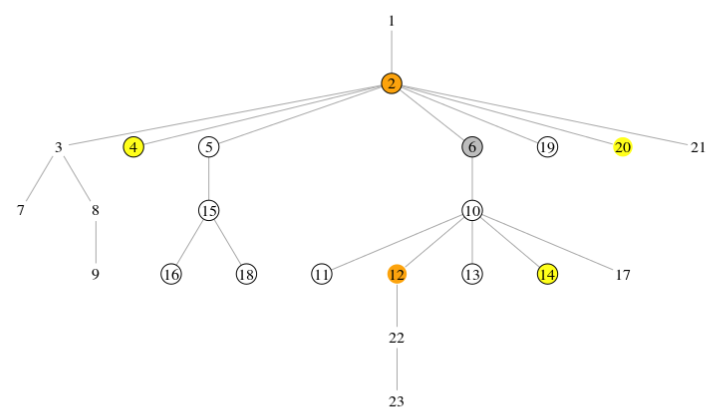
\includegraphics[width=1\textwidth]{breakpoints2}
	\end{figure}
\end{frame}


\begin{frame}{Time-based neighbourhoods}{Census}
We found 165 different motifs:
	\begin{figure}
		\centering
		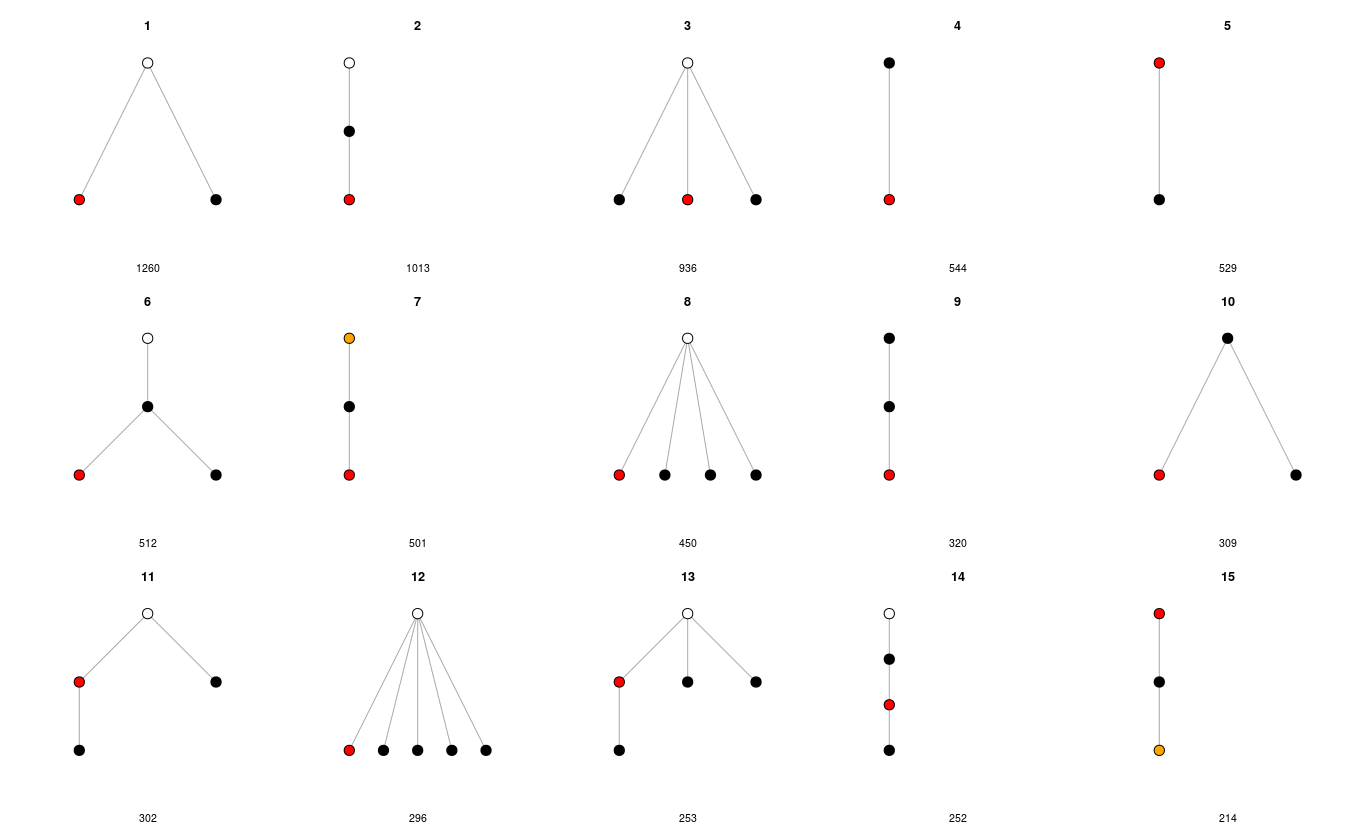
\includegraphics[width=1\textwidth]{neighbourhoods_time_1}
	\end{figure}
\end{frame}

\section{Conversation-based clustering}
\begin{frame}{Methodology}
	\begin{itemize}
	\item Create a user $\times$ neighborhood matrix of counts.
	\item Z-normalize (users characterized by their deviation from the mean)
	\item Cluster!
\end{itemize}
\end{frame}

\begin{frame}{Conversation-based clustering}{Order-based}
	\begin{figure}
		\centering
		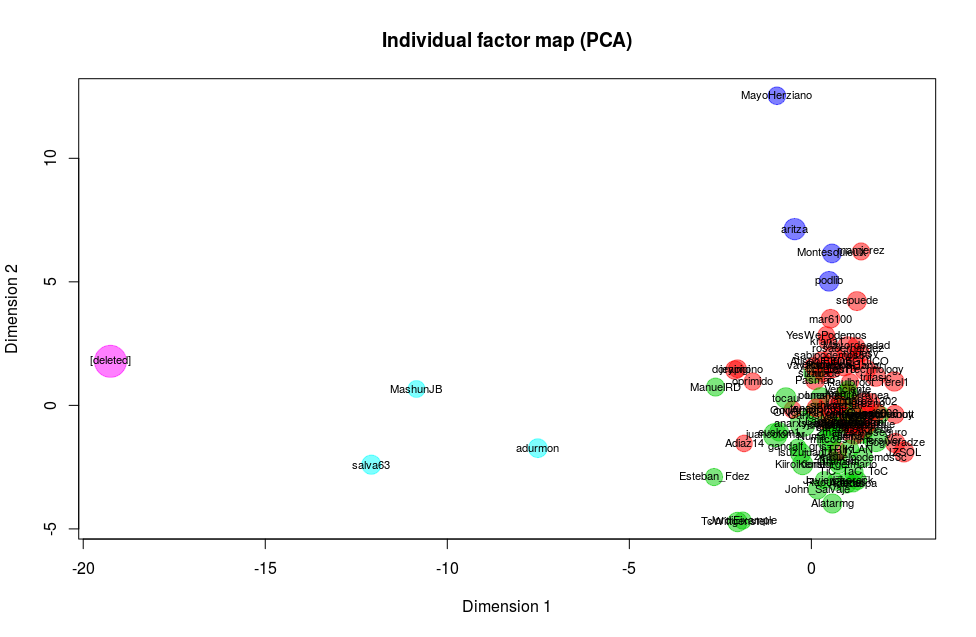
\includegraphics[width=1\textwidth]{PCA_cluster_order_based}
	\end{figure}	
\end{frame}


\section{Conclusions}
\begin{frame}{Conclusions}
	\begin{itemize}
	\item \textbf{Q: Can we use graph structure to characterise users?}
	\item A: Yes!
	\end{itemize}	
	\begin{itemize}
	\item \textbf{Q: By using triads}?
	\item A: No. They are not useful in trees.
	\end{itemize}
	\begin{itemize}
	\item \textbf{Q: So, what kind of structure?}
	\item A: Posts neighbourhoods that are time/order sensitive.
	\end{itemize}
	\begin{itemize}
	\item \textbf{Q: What about language?}
	\item A: It's ok, but structure is more directly linked to thread dynamics (future work)
	\end{itemize}
	\textbf{Future work:}
	\begin{itemize}
		\item Prune time-based neighbourhoods to reduce dimensionality.
		\item Do users jump from cluster to cluster (paths of roles)
	\end{itemize}	
\end{frame}

\begin{frame}
\begin{center}
\Huge Merci !
	\begin{figure}
		\centering
		%
\includegraphics[width=0.1\textwidth]{reddit-logo}
		%
\includegraphics[width=0.2\textwidth]{reddit_french}	
		%
\includegraphics[width=0.5\textwidth]{reddit_questions}
		
\includegraphics[width=0.1\textwidth]{reddit_sans_culotte}
	\end{figure}
\end{center}
\end{frame}
\end{document}